\documentclass{standalone}
\usepackage{tikz}
\usepackage{pgfmath}
\usetikzlibrary{shadings}

\begin{document}

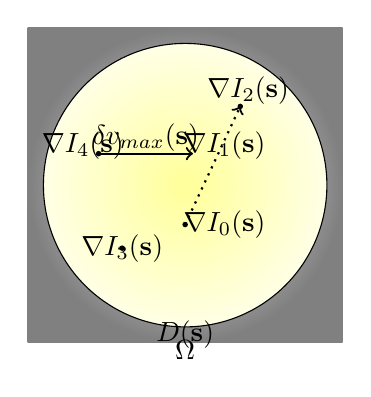
\begin{tikzpicture}

% Background shading
\shade[inner color=white, outer color=gray] (-2,-2) rectangle (2,2);

% Circle shading
\shade[inner color=yellow!40, outer color=yellow!10] (0,0) circle (1.8);

% Circle boundary
\draw (0,0) circle (1.8);

% Labels and gradients
\node at (-1.3,0.5) {$\nabla I_4(\mathbf{s})$};
\node at (0.5,0.5) {$\nabla I_1(\mathbf{s})$};
\node at (0.8,1.2) {$\nabla I_2(\mathbf{s})$};
\node at (0.5,-0.5) {$\nabla I_0(\mathbf{s})$};
\node at (-0.8,-0.8) {$\nabla I_3(\mathbf{s})$};

% Dotted line and arrow
\draw[->, thick, dotted] (0,-0.5) -- (0.7,1);

% Delta vmax label
\draw[->, thick] (-1.1,0.4) -- (0.1,0.4);
\node at (-0.5,0.6) {$\delta v_{\text{max}}(\mathbf{s})$};

% Region labels
\node at (0,-2.1) {$\Omega$};
\node at (0,-1.9) {$D(\mathbf{s})$};

% Points
\fill (0,-0.5) circle (1pt);
\fill (0.7,1) circle (1pt);
\fill (-1.1,0.4) circle (1pt);
\fill (-0.8,-0.8) circle (1pt);

\end{tikzpicture}

\end{document}